\documentclass[12pt]{article}

\usepackage{sbc-template}
\usepackage{graphicx,url}
\graphicspath{{images/}}

\usepackage[brazil]{babel}
\usepackage[latin1]{inputenc}

\usepackage[alf,bibjustif,abnt-full-initials=no,abnt-etal-cite=2,abnt-and-type=1,abnt-etal-text=it,abnt-url-package=url,abnt-emphasize=bf]{abntcite}%[alf]{abntcite}

\usepackage{float}
\usepackage{subfigure}

\sloppy

\title{Comparativo de protocolos de roteamento em redes \textit{ad hoc} m\'oveis em cen\'arios militares.}
\author{
	F\'abio Leandro Janiszevski\inst{1}, 
	Dr. Daniel Kikuti\inst{1}, 
	Ms. Hermano Pereira\inst{2}
}
\address{
	Universidade Estadual do Centro-Oeste - UNICENTRO
\nextinstitute
	Universidade Tecnol\'ogica Federal do Paran\'a - UTFPR
\email{
	fabiosammy@gmail.com,
	danielkikuti@yahoo.com.br,
	hermanopereira@utfpr.edu.br}
}

\begin{document}
\maketitle

\begin{abstract}
This article presents a study of different routing protocols in ad hoc networks, analyzing the performance in military scenarios, making comparisons between them through simulations with the NS-2 tool.
Where we used the protocols DSDV, and OLSR AODL in 2 different scenarios, of which we can analyze the performance a little of each.
\end{abstract}

\begin{keyWord}
Ad hoc networks; military scenarios, routing protocols, AODV, DSDV, OLSR;
\end{keyWord}

\begin{resumo}
Este artigo apresenta um estudo de diferentes protocolos de roteamento em redes ad hoc, analizando a performance em cen\'arios militares, realizando compara\c{c}\~oes entre os mesmos atrav\'es de simula\c{c}\~oes com a ferramenta NS-2. 
Onde foram utilizados os protocolos DSDV, AODL e OLSR em 2 diferentes cen\'arios, dos quais podemos analizar um pouco o desempenho de cada um.
\end{resumo}

\begin{palavraChave}
Redes ad hoc; Cen\'arios militares; Protocolos de roteamento; AODV; DSDV; OLSR;
\end{palavraChave}

\section{Introdu\c{c}\~ao} 
Atualmente, a maioria da popula\c{c}\~ao possui um dispositivo port\'atil com disponibilidade de conex\~ao em redes sem-fio e capaz de se comunicar com outros dispositivos. 
Com a populariza\c{c}\~ao destes dispositivos, \'e muito comum existirem in\'umeras redes sem-fio dispon\'iveis para conex\~ao abertamente, ou a possibilidade de se criar uma nova conforme necessidade.

As redes sem-fio (chamadas de \textit{wireless}), prov\^em comunica\c{c}\~ao, seja com uma pequena ou grande rede de comunica\c{c}\~ao. 
Essas redes podem ser classificadas em:

\begin{itemize}
	\item Redes infra-estruturadas.
	\item Redes \textit{ad hoc}.
\end{itemize}

Nas redes infra-estruturadas, toda a comuni\c{c}\~ao entre os n\'os m\'oveis \'e feita pelo meio de uma Esta\c{c}\~ao de Suporte \`a Mobilidade (ESM) na rede fixa.
A ESM gera sinal oferecendo acesso aos \textit{hosts}, e os \textit{hosts} s\'o geram conex\~oes, aplica\c{c}\~oes dos usu\'arios. Quem gera as rotas, o roteador, \'e a ESM. 

As redes \textit{ad hoc} s\~ao chamadas de MANET(\textit{Mobile ad hoc network}), pois n\~ao \'e necess\'ario uma estrutura fixa para que a comunica\c{c}\~ao funcione.
No tipo de rede infra-estruturada, os n\'os m\'oveis, mesmo pr\'oximos um do outro, est\~ao impossibilitados de estabelecer comunica\c{c}\~ao direta entre si \cite{pereira}.

As MANETs n\~ao possuem a ESM, elas t\^em uma dinamicidade grande em sua forma de comunica\c{c}\~ao, pois cada novo n\'o na rede, atuar\'a como um roteador e como um \textit{host}, executando aplica\c{c}\~oes dos usu\'arios. 
Existem poucos protocolos oficiais de roteamento para as redes \textit{ad hoc}, pois  o roteamento nesse tipo de rede \'e um grande desafio devido a forma din\^ amica de como a topologia da rede \'e desenvolvida.

Os autores \cite{pepe} comentam sobre a dinamicidade das redes \textit{ad hoc} e a facilidade em criar uma rede dessas.
As MANETs proporcionam estruturas de comunica\c{c}\~ao em ambientes com obst\'aculos \`a cria\c{c}\~ao de uma estrutura fixa.
Um cen\'ario de opera\c{c}\~ao militar pode ser visto como uma situa\c{c}\~ao em que as MANETs s\~ao requiridas para viabilizar a comunica\c{c}\~ao em um ambiente hostil e geograficamente acidentado, n\~ao possibilitando a exist\^encia de uma estrutura fixa \cite{schimidt}.

Segundo \cite{salles}, a necessidade de uma comunica\c{c}\~ao r\'apida em uma equipe militar \'e essencial para obte\c{c}\~ao de sucesso em operac\~oes, pois qualquer atraso na comunicac\~ao pode desencadear um final catastr\'ofico na execuc\~ao da opera\c{c}\~ao. 
Os diversos protocolos existentes das redes \textit{ad hoc} diferenciam-se em: n\'umero de pacotes de requisic\~oes a transitar na rede, modo de atualizac\~ao das rotas, sistema de armazenamento de rotas, e outros. Portanto a escolha do protocolo de roteamento pode influenciar no desempenho final da rede.

O objetivo deste artigo \'e apresentar um estudo de diferentes protocolos de roteamento em redes \textit{ad hoc} em cen\'arios militares, atrav\'es de m\'etricas de performance baseados em estudos realizados por \cite{pereira} e \cite{salles}.
		%Introdução
%\section{Hist\'orico}
\subsection{Redes \textit{wireless}}
\subsection{O padr\~ ao IEEE 802.11}
		%Histórico
\section{Protocolos de roteamento em redes \textit{ad hoc}}
Em redes m\'oveis \textit{ad hoc}, uma rota entre dois n\'os pode ser formada por v\'arios saltos atrav\'es de um ou mais n\'os na rede. 

Os protocolos s\~ao variados, mas segundo \cite{gorantala}, somente dois s\~ao de suma import\^ancia da rede, o DSDV(\textit{Destination Sequenced Distance Vector}), para redes pequenas, e o AODV(\textit{Ad-hoc On-Demand Distance Vector}), para redes \textit{ad hoc} em geral. 
Cada protocolo trabalha de uma forma diferente, em que estes podem ser classificados em pr\'o-ativo ou reativo. 
"Os protocolos pr\'o-ativos mant\^em rotas para todos os n\'os da rede, independente do uso ou necessidade destas rotas. (...) J\'a os protocolos reativos iniciam as atividades de roteamento de acordo com a demanda" \cite{pereira}.

Os roteadores em uma rede \textit{ad hoc} trocam informa\c{c}\~oes de roteamento uns com os outros com a finalidade de tomar conhecimento das disponibilidades de rotas e da topologia da rede.\cite{pereira}

%Arrumar
\textit{Abaixo citei tudo \cite{gorantala}}

\subsection{\textit{Destination sequenced distance vector} - DSDV}\label{subDSDV} 
O protocolo DSDV \'e um protocolo de roteamento pr\'o-ativo\cite{gorantala}, baseado no algoritmo de vetor de dist\^ancias, que trabalha requisitando periodicamente, de cada um dos n\'os vizinhos, suas tabelas de roteamento, com a finalidade de mant\^e-las atualizadas. 
Cada n\'o da rede mant\'em uma tabela de roteamento, contendo o pr\'oximo salto e o n\'umero de saltos para cada destino alcan\c{c}\'avel. 
As tabelas incluem rotas para todos os n\'os da rede, mesmo que nunca seja necess\'ario enviar pacote para este n\'o. 
Cada n\'o mant\'em apenas uma rota para cada destino.

Os \textit{loops} de rotas podem ocorrer quando informa\c{c}\~oes de roteamento incorretas s\~ao mantidas na rede ap\'os uma troca de topologia. 
Geralmente, ocorre quando um n\'o detecta uma queda no enlace com o n\'o vizinho e, antes que consiga propagar sua nova tabela, recebe de outro n\'o informa\c{c}\~ao desatualizada referente \`a conex\~ao interrompida. 
A vantagem principal do DSDV sobre os protocolos baseados em Vetor de Dist\^ancias tradicionais \'e que ele garante a aus\^encia de \textit{loops}, usando o conceito de n\'umero de sequ\^encia mantido em cada rota. 
O n\'umero de sequ\^encia \'e estabelecido pelo n\'o destino e \'e incrementado a cada novo aviso de rota.
As rotas mais recentes possuem um n\'umero de sequ\^encia maior e s\~ao as mais favor\'aveis. 
Caso os n\'umeros de sequ\^encia sejam iguais, a rota que tiver o menor n\'umero de saltos ser\'a a mais favor\'avel. 
Neste contexto, o uso de n\'umeros de sequ\^encia faz com que o DSDV se adapte melhor para redes de topologia din\^amica como redes \textit{ad hoc}.

\subsubsection{Exemplo de funcionamento do DSDV}

A Figura \ref{figOpDSDV}, descreve uma rede com 8 hosts. 
Pode-se analisar a mudan\c{c}a de roteamento da tabela do MH4 em rela\c{c}\~ao ao movimento do \textit{host} MH1(\textit{Mobile Host} 1), onde o movimento \'e representado pelas setas com estilo pontilhado. 

\begin{figure}[H]
	\centering
	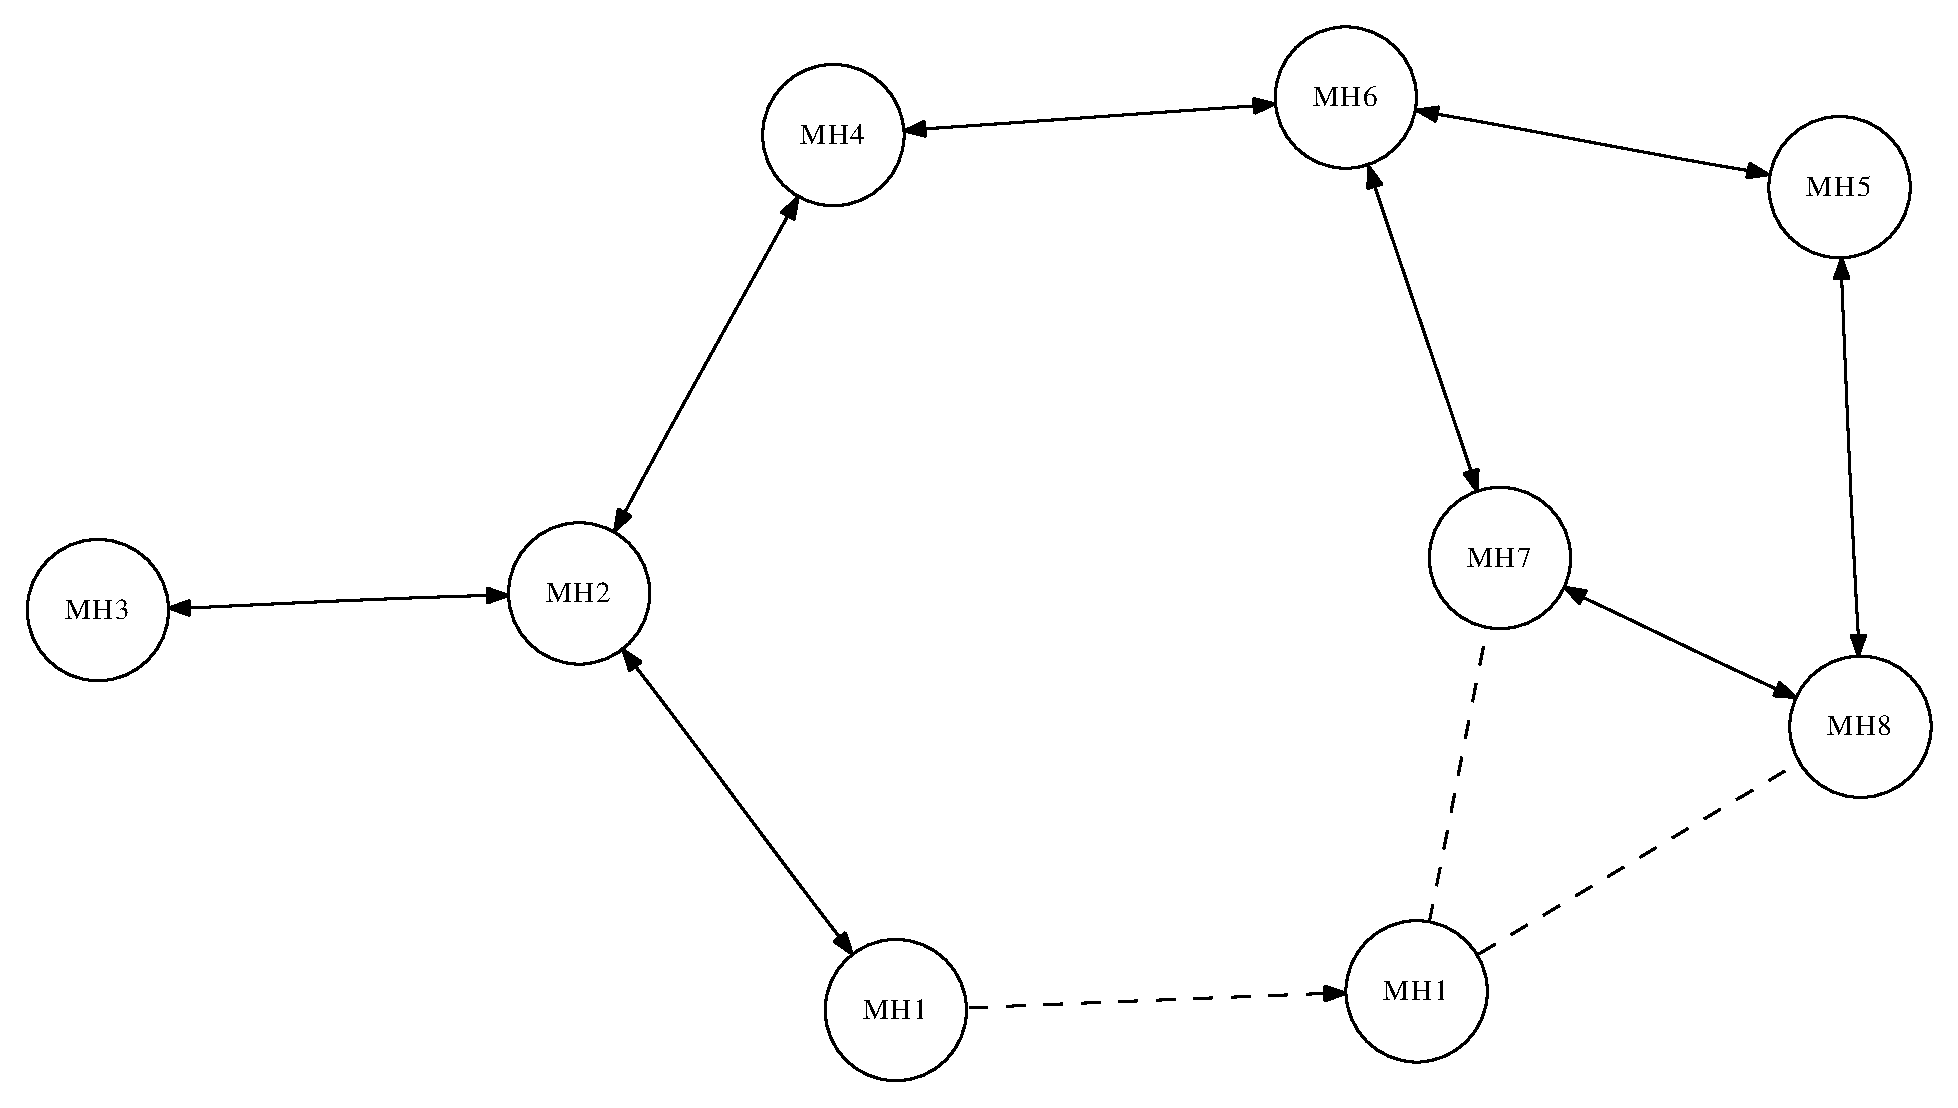
\includegraphics[scale=.4]{dsdvOperation.eps}
	\caption{Exemplo de opera\c{c}\~ ao do DSDV}
	\label{figOpDSDV}
\end{figure}

Uma tabela de roteamento do DSDV, cont\'em, para cada n\'o na rede:
\begin{itemize}
	\item Informa\c{c}\~oes do n\'o de destino;
	\item o pr\'oximo salto na rota para alcan\c{c}ar o destino;
	\item a m\'etrica com o valor de quantos saltos s\~ao necess\'arios para alcan\c{c}ar o destino;
	\item o n\'umero de sequ\^encia utilizado para sincroniza\c{c}\~ao das rotas;
	\item o install, atuando como um marcador de tempo da rota, para decidir de deletar ou n\~ao uma nova informa\c{c}\~ao topol\'ogica; e
	\item o campo informa\c{c}\~ao, servindo como um ponteiro para indicar a tabela com informa\c{c}\~oes sobre a estabilidade da rota.
\end{itemize}

Inicialmente, todos os n\'os anunciam suas informa\c{c}\~oes de roteamento para todos os outros n\'os da rede e, portanto, a tabela de roteamento do \textit{host} MH4 inicialmente apresenta o seguinte conte\'udo conforme a Tabela \ref{tabRtMH4}.

\begin{table}[H]
	\centering
	\caption{Tabela de roteamento do \textit{host} MH4 \cite{pebha}}
	\begin{tabular}{ | c | c | c | c | c | c | }
		\hline
		Destino & Pr\'oximo salto & M\'etrica & N\'umero de sequ\^encia & Install & Informa\c{c}\~ao \\ \hline
		MH1 & MH2 & 2 & S406\_MH1 & T001\_MH4 & Ptr1\_MH1 \\ \hline
		MH2 & MH2 & 1 & S128\_MH2 & T001\_MH4 & Ptr1\_MH2 \\ \hline
		MH3 & MH2 & 2 & S564\_MH3 & T001\_MH4 & Ptr1\_MH3 \\ \hline
		MH4 & MH4 & 0 & S710\_MH4 & T001\_MH4 & Ptr1\_MH4 \\ \hline
		MH5 & MH6 & 2 & S309\_MH5 & T002\_MH4 & Ptr1\_MH5 \\ \hline
		MH6 & MH6 & 1 & S076\_MH6 & T001\_MH4 & Ptr1\_MH6 \\ \hline
		MH7 & MH6 & 2 & S128\_MH7 & T002\_MH4 & Ptr1\_MH7 \\ \hline
		MH8 & MH6 & 3 & S050\_MH8 & T002\_MH4 & Ptr1\_MH8 \\ \hline
	\end{tabular}
	\label{tabRtMH4}
\end{table}

Por\'em, quando o \textit{host} MH1 move sua localiza\c{c}\~ao para pr\'oximo dos \textit{hosts} MH7 e MH8 como apresentado na Figura \ref{figOpDSDV} ent\~ao, o enlace entre MH2 e MH1 vai ser quebrado.
Isto resulta em atribui\c{c}\~ao de uma m\'etrica infinita de MH2 para MH1 e o n\'umero de sequ\^encia ser\'a alterado para um n\'umero \'impar na tabela de roteamento em MH2, que atualizar\'a essa informa\c{c}\~ao para os \textit{hosts} vizinhos. 
Desde que haja um novo \textit{host} vizinho para MH7 e MH8, eles v\~ao atualizar essa informa\c{c}\~ao nas respectivas tabelas de roteamento e propagar essa nova informa\c{c}\~ao. 
Agora, MH4 receber\'a esta atualiza\c{c}\~ao de informa\c{c}\~ao de MH6, onde MH6 recebe 2 pacotes de informa\c{c}\~oes de diferentes vizinhos para chegar em MH1 com o mesmo n\'umero de sequ\^encia, mas com diferentes m\'etricas. 
A sele\c{c}\~ao da rota ir\'a depender da menor contagem de saltos quando o n\'umero de sequ\^encia \'e o mesmo. 
A tabela de roteamento do MH4 estar\'a com o conte\'udo demonstrado na Tabela  \ref{tabNewRtMH4}.

\begin{table}[H]
	\centering
	\caption{Tabela de roteamento do \textit{host} MH4 depois do movimento do \textit{host} MH1 \cite{pebha}}
	\begin{tabular}{ | c | c | c | c | c | c | }
		\hline
		Destino & Pr\'oximo salto & M\'etrica & N\'umero de sequ\^encia & Install & Informa\c{c}\~ao \\ \hline
		MH1 & MH6 & 3 & S516\_MH1 & T001\_MH4 & Ptr1\_MH1 \\ \hline
		MH2 & MH2 & 1 & S238\_MH2 & T001\_MH4 & Ptr1\_MH2 \\ \hline
		MH3 & MH2 & 2 & S674\_MH3 & T001\_MH4 & Ptr1\_MH3 \\ \hline
		MH4 & MH4 & 0 & S820\_MH4 & T001\_MH4 & Ptr1\_MH4 \\ \hline
		MH5 & MH6 & 2 & S502\_MH5 & T002\_MH4 & Ptr1\_MH5 \\ \hline
		MH6 & MH6 & 1 & S186\_MH6 & T001\_MH4 & Ptr1\_MH6 \\ \hline
		MH7 & MH6 & 2 & S238\_MH7 & T002\_MH4 & Ptr1\_MH7 \\ \hline
		MH8 & MH6 & 3 & S160\_MH8 & T002\_MH4 & Ptr1\_MH8 \\ \hline
	\end{tabular}
	\label{tabNewRtMH4}
\end{table}

\subsubsection{Vantagens do DSDV}
\begin{itemize}
	\item Livre de \textit{loops} \cite{gorantala}.
	\item Problemas com contagem ao infinito \'e reduzido no DSDV \cite{gorantala}.
	\item Pode-se evitar tr\'afego extra com atualiza\c{c}\~oes incrementais, em vez de atualiza\c{c}\~oes de despejo completo.
	\item Sele\c{c}\~ao de caminho: O DSDV mant\'em somente o melhor caminho em vez de manter v\'arios caminhos para um mesmo destino. Com isso, o espa\c{c}o da tabela de roteamento \'e reduzido.
\end{itemize}

\subsubsection{Limita\c{c}\~ oes do DSDV}
\begin{itemize}
	\item Desperd\'icio do uso da banda na rede devido \`a propaga\c{c}\~ao desnecess\'aria de informa\c{c}\~oes de roteamento, mesmo se n\~ao houver mudan\c{c}as na topologia da rede \cite{Patel00energyin}.	
	\item O DSDV n\~ao suporta m\'ultiplos caminhos de rotas \cite{gorantala}.
	\item \'E dif\'icil determinar um tempo de converg\^encia para a propaga\c{c}\~ao das rotas \cite{heg}.
	\item \'E dif\'icil manter a propaga\c{c}\~ao das tabelas de rotas para uma grande rede. Cada \textit{host} na rede deve manter uma tabela de rotas para propaga\c{c}\~ao. Mas para uma grande rede, isso causaria \textit{overhead} de rede, o qual consome uma maior banda na rede \cite{gorantala}.
\end{itemize}
	%Destination sequenced distance vector - DSDV
\subsection{\textit{Ad hoc on demand distance vector} - AODV}
O protocolo AODV \'e um protocolo reativo, baseado em vetor de dist\^ancias, e pode ser considerado como uma combina\c{c}\~ao de outros dois protocolos, denominados DSR e DSDV. 
O AODV tem a base do DSR, o qual \'e baseado sob demanda, ou seja, descobre rotas somente quando necess\'ario, e utiliza os mecanismos de descoberta de rotas e manuten\c{c}\~ao de rotas.
Entretando, o AODV utiliza a caracter\'istica do DSDV de obrigar todos os n\'os intermedi\'arios a estabelecerem dinamicamente entradas em tabelas de roteamento locais para cada destino ativo.
Cada n\'o tem conhecimento do pr\'oximo salto para alcan\c{c}ar o destino e a dist\^ancia em n\'umero de saltos.
Pode ser considerado como uma vers\~ao melhorada do DSDV, uma ver que seu funcionamento baseado em demanda minimiza o n\'umero de inunda\c{c}\~oes na rede exigido pelo DSDV para cria\c{c}\~ao de rotas.

\subsubsection{Limita\c{c}\~oes e desvantagens do AODV}
\begin{description}
	\item[Necessidade de um meio de propaga\c{c}\~ ao:] O algoritmo necessita que os n\'os no meio da propaga\c{c}\~ ao possam detectar outros 
	\item[N\~ao reutiliza informa\c{c}\~oes de roteamento] O AODV carede de efici\^encia na t\'ecnica de manuten\c{c}\~ao de suas rotas. Informa\c{c}\~oes de roteamento s\~ao sempre atualizadas em cada demanda, inclu\'indo casos comuns de tr\'afego. \cite{ramachandran}
\end{description}
	%Ad hoc on demand distance vector} - AODV
\subsection{\textit{Optimized link state routing} - OLSR}
O protocolo OLSR \cite{rfc3626} \'e um protocolo pr\'o-ativo, baseado em estado de conex\~ao, onde cada n\'o possui as informa\c{c}\~oes de rotas e compartilham entre si constantemente. 
O diferencial desse protocolo em rela\c{c}\~ao ao DSDV, que tamb\'em \'e pro-\'ativo, por\'em baseado em dist\^ancia de vetores, \'e que o OLSR diminui o tr\'afego de informa\c{c}\~oes de roteamento utilizando somente alguns n\'os pr\'e-selecionados, para retransmitir as mensagens de descoberta de rotas na rede.
Essa t\'ecnica \'e denominada MPR (\textit{Multipoint Relay}).

\subsubsection{Exemplo de funcionamento do OLSR}
Considerando as Figuras \ref{fig:olsrComum} e \ref{fig:olsrOperation}, temos a diferen\c{c}a de funcionamento de descoberta de rotas a cada passo, onde cada n\'o repassa as informa\c{c}\~oes de rotas entre os n\'os vizinhos.

\begin{figure}[H]
	\centering
	\subfigure[Primeiro est\'agio]{
		\includegraphics[scale=0.3]{olsrOperationStep1.eps}
	}\label{subfig:olsrStep11}
	\subfigure[Segundo est\'agio]{
		\includegraphics[scale=0.3]{olsrOperationStep2.eps}
	}\label{subfig:olsrStep12}
	\subfigure[Terceiro est\'agio]{
		\includegraphics[scale=0.3]{olsrOperationStep3.eps}
	}\label{subfig:olsrStep13}
	\subfigure[Quarto est\'agio]{
		\includegraphics[scale=0.3]{olsrOperationStep4.eps}
	}\label{subfig:olsrStep14}	
	\caption{Descoberta de rotas do protocolo DSDV}
	\label{fig:olsrComum}
\end{figure}

O mecanismo para selecionar os vizinhos que ir\~ao retransmitir os pacotes, denominado MPR, \'e simples. Ele escolhe vizinhos alcan\c{c}\'aveis atrav\'es de um salto que tenham comunica\c{c}\~ao sim\'etrica, bidirecional, com pacotes de mensagens \textit{HELLO}

\begin{figure}[H]
	\centering
	\subfigure[Primeiro est\'agio]{
		\includegraphics[scale=0.3]{olsrOperationStep1.eps}
	}\label{subfig:olsrStep21}
	\subfigure[Segundo est\'agio]{
		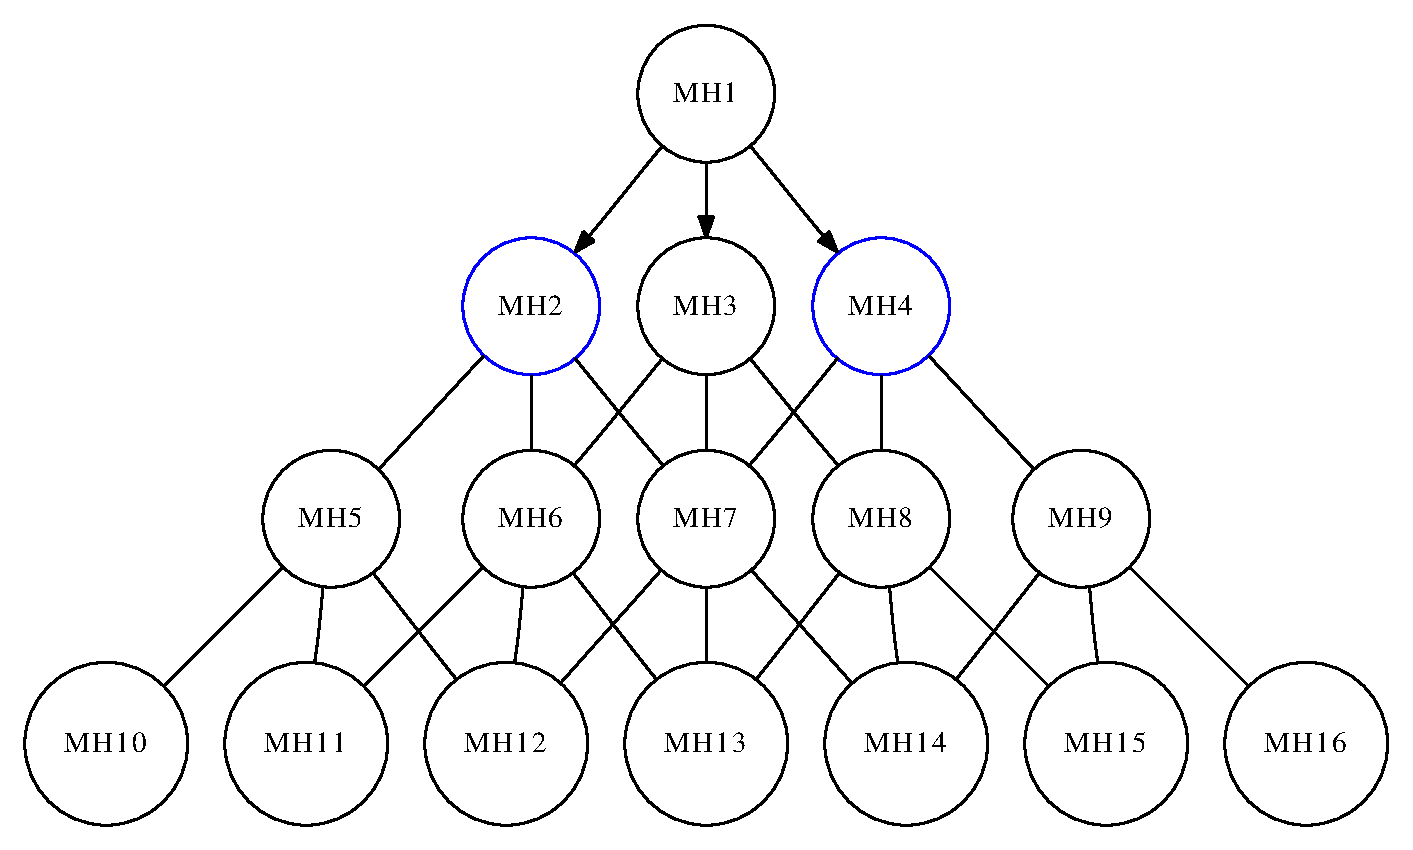
\includegraphics[scale=0.3]{olsrOperationStep5.eps}
	}\label{subfig:olsrStep22}
	\subfigure[Terceiro est\'agio]{
		\includegraphics[scale=0.3]{olsrOperationStep6.eps}
	}\label{subfig:olsrStep23}
	\subfigure[Quarto est\'agio]{
		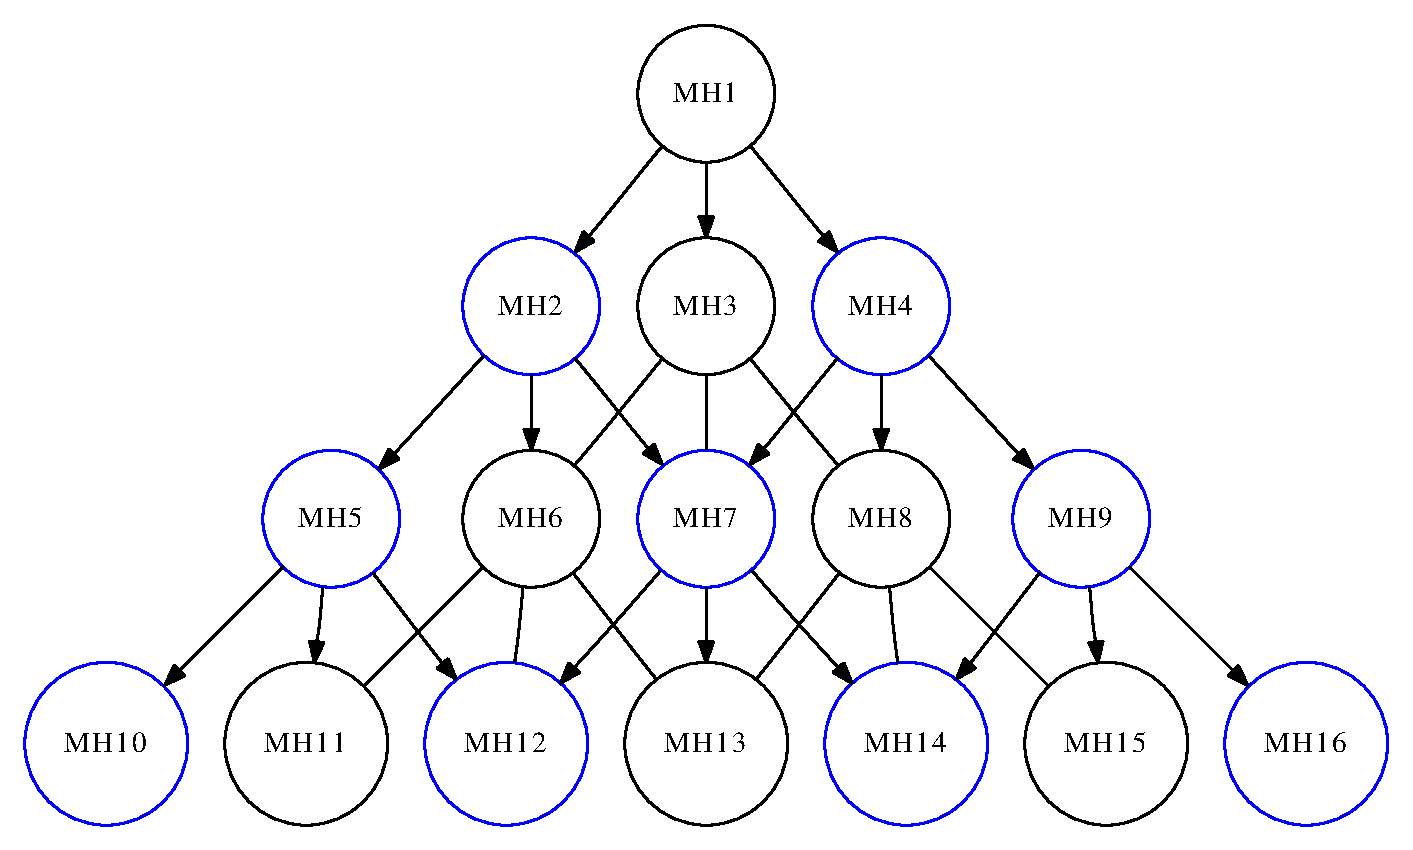
\includegraphics[scale=0.3]{olsrOperationStep7.eps}
	}\label{subfig:olsrStep24}	
	\caption{Descoberta de rotas do protocolo OLSR}
	\label{fig:olsrOperation}
\end{figure}


	%Optimized link state routing - OLSR
		%Protocolos de roteamento em redes ad hoc
\section{Metodologia dos testes} 
Neste trabalho, o objetivo das simula\c{c}\~oes \'e permitir uma an\'alise do comportamento de tr\^es protocolos de roteamento em redes \textit{ad hoc} (AODV, DSDV e OLSR), sob a influ\^encia de dois cen\'arios que retratam uma aplica\c{c}\~ao militar, revelando os problemas decorrentes da utiliza\c{c}\~ao deste tipo de rede em um cen\'ario com essas caracter\'isticas, e buscando as melhores condi\c{c}\~oes para contornar estes problemas. 
Al\'em disso, por meio das simula\c{c}\~oes realizadas podemos avaliar o impacto que a mobilidade em grupo, a configura\c{c}\~ao de rede hier\'arquica e o movimento dos n\'os em uma dire\c{c}\~ao pr\'e-determinada podem causar no roteamento dos dados.

\subsection{Ambiente de simula\c{c}\~ ao}
Para o trabalho apresentado, os testes s\~ao baseados em um simulador desenvolvido em um projeto colaborativo entre a Universidade da Calif\'ornia do Sul e o laborat\'orio Xerox PARC, o simulador NS-2 \cite{FallVaradhan}.

O NS-2 \'e um simulador de eventos discreto, oferecendo suporte \`a simula\c{c}\~ao de um grande n\'umero de topologias de redes diferentes cen\'arios baseados nos protocolos TCP e UDP, diversos escalonadores e pol\'iticas de fila, caracteriza\c{c}\~ao de tr\'afego com diversas distribui\c{c}\~oes estat\'isticas dentre outras finalidades.

\subsection{Cen\'arios militares}
Segundo \cite{pereira}, em um cen\'ario de opera\c{c}\~oes militares \'e indispens\'avel o uso de tecnologias de comunica\c{c}\~ao sem fio. 
Principalmente das tecnologias que tenham capacidade de atuar de forma aut\^onoma e proporcionar qualidade de conex\~ao juntamente com o grau de dinamicidade na topologia da rede.
A qualidade da rede de comuni\c{c}\~ao utilizada em uma opera\c{c}\~ao militar pode acarretar o sucesso ou fracasso da miss\~ao.

\subsubsection{Requisitos b\'asicos}
Segundo \cite{salles}, v\'arios requisitos s\~ao necess\'arios para que uma rede \textit{ad hoc} possa funcionar efetivamente em um cen\'ario real militar, onde o autor enumera v\'arios princ\'ipios de emprego das comunica\c{c}\~oes militares no Ex\'ercito Brasileiro, que s\~ao:
\begin{description}
	\item[Tempo integral:] Operar 24 horas por dia, todos os dias.
	\item[Rapidez:] Estabelecer contato em tempo \'util para surtir os efeitos desejados.
	\item[Amplitude de desdobramento:] Estar operacional em todo o teatro de opera\c{c}\~oes.
	\item[Integra\c{c}\~ao:] Operar junto com os sistemas dos escal\~oes superior e inferior.
	\item[Flexibilidade:] Adequar-se rapidamente \`as mudan\c{c}as das opera\c{c}\~oes t\'aticas e das oraganiza\c{c}\~oes militares.
	\item[Apoio em profundidade:] Apoio ao escal\~ao superior (mais recuado) para com os escal\~oes subordinados (mais avan\c{c}ado).
	\item[Continuidade:] Retomar as comunica\c{c}\~oes e mant\^e-las a qualquer custo, mesmo que o escal\~ao considerado n\~ao seja o respons\'avel.
	\item[Confiabilidade:] Estar sempre dispon\'ivel, estabelecendo caminhos alternativos para a transmiss\~ao das mensagens.
	\item[Emprego centralizado:] Concentrar meios em centros e eixos de comunica\c{c}\~oes permitindo melhor aproveitamento dos mesmos.
	\item[Apoio cerrado:] Encurtar as dist\^ancias sempre que poss\'ivel para facilitar as comunica\c{c}\~oes.
	\item[Seguran\c{c}a:] Impedir ou pelo menos dificultar a obten\c{c}\~ao da informa\c{c}\~ao pelo inimigo.
	\item[Prioridade:] Estabelecer comunica\c{c}\~ao e transmitir mensagens de acordo com a prioridade preestabelecida.
\end{description}

Esses mesmos princ\'ipios foram mapeados pelos autores \cite{salles} em outros cinco outros termos utilizados comumente na concep\c{c}\~ao de redes de comunica\c{c}\~oes. Abaixo a tabela \ref{tabExer} demonstra o mapeamento.
\begin{table}[H]
	\centering
	\caption{Mapeamento em princ\'ipios gerais dos princ\'ipios de emprego das comunica\c{c}\~oes militares no Ex\'ercito Brasileiro \cite{salles}}
	\begin{tabular}{ | l | l | }
		\hline
		\textbf{Princ\'ipios gerais} & \textbf{Princ\'ipios de emprego das comunica\c{c}\~oes militares} \\ \hline
		Escalabilidade & Amplitude de desdobramento, Integra\c{c}\~ao. \\ \hline
		Desempenho & Tempo integral, Rapidez, Confiabilidade, Continuidade, Prioridade \\ \hline
		Seguran\c{c}a & Seguran\c{c}a \\ \hline
		Gerenciabilidade & Apoio em profundidade, Emprego centralizado, Apoio cerrado \\ \hline
		Usabilidade & Flexibilidade \\ \hline
	\end{tabular}
	\label{tabExer}
\end{table}

\textit{Fazer rela\c{c}\~ao dos dados com o objetivo desempenho}

\subsubsection{Movimenta\c{c}\~ao}

\subsection{Tr\'afego de dados}\label{trafegoDados}
Para obter uma compara\c{c}\~ao justa entre todos os protocolos, \'e necess\'ario selecionar um agente que n\~ao crie condi\c{c}\~oes de desigualdade, como mecanismos pr\'oprios de controle de congestionamento.
O simulador utilizado, NS-2, oferece a possibilidade de gerar conex\~oes de tr\'afego TCP(\textit{Transport Control Protocol}) ou CBR(\textit{Constant Bit Rate}).
O documento \cite{rfc793} define que o TCP possui um mecanismo pr\'oprio de controle de congestionamento, e tamb\'em os pacotes de reconhecimento (ACK) do agente disputam o canal, podendo causar colis\~oes e degradar o desempenho.
Com base nisso, o CBR(\textit{Constant Bit Rate}) foi selecionado, o qual usa agente UDP(\textit{User Datagram Protocol}), que n\~ao possui um controle de congestionamento pr\'oprio \cite{rfc768}.
	%Metodologia dos testes
\section{Experimentos e resultados}\label{experimentos}
\subsection{Experimentos}
Para compreender o funcionamento do simulador NS-2 e tamb\'em estudar simula\c{c}\~oes de comunica\c{c}\~ao em cen\'arios militares, foram definidos dois experimentos te\'oricos, sendo o Experimento 1, um teste simples de converg\^encia de rotas, e o Experimento 2, baseado em estudos realizados por \cite{pereira}, o qual representa um caso de assalto e tomada de posi\c{c}\~ao inimiga.

Cada experimento possui suas caracter\'isticas, mas exite uma semelhan\c{c}a base, que \'e o tr\'afego que ir\'a caminhar pela rede, como comentado na se\c{c}\~ao \ref{trafegoDados}, o qual foi escolhido o CBR.

\subsubsection{Experimento 1}
O Experimento 1 baseia-se na ideia simples de um protocolo de rede \textit{ad hoc}, roteamento din\^amico.
O objetivo principal deste experimento \'e poder analisar o tempo de converg\^encia de roteamento de uma origem a um destino, alterando uma vez o caminho pelo qual eles realizam a comunica\c{c}\~ao.
A Tabela \ref{tabParamExp1} demonstra resumidamente os par\^ametros utilizados na execu\c{c}\~ao do Experimento 1.

\begin{table}[H]
	\centering
	\caption{Resumo dos par\^ametros usados no Experimento 1.}
	\begin{tabular}{ | l | l | }
		\hline
		N\'umero total de n\'os & 4 \\ \hline
		N\'umero de fontes de tr\'afego & 1 \\ \hline
		N\'umero de conex\~oes & 1 \\ \hline
		Tempo de simula\c{c}\~ao & 300 segundos \\ \hline
		\'Area total da simula\c{c}\~ao & 500x500 metros \\ \hline
		Tamanho dos pacotes & 512 \textit{bytes} \\ \hline	
		Velocidade dos n\'os & 1.5m/s constante \\ \hline
		Velocidade de banda & 11Mbps/s \\ \hline
	\end{tabular}
	\label{tabParamExp1}
\end{table}

A Figura \ref{figExp1} demonstra o experimento realizado, onde cada Soldado(n\'o) deve atingir seu respectivo Destino.
Cada Soldado inicia seu movimento a um tempo determinado na simula\c{c}\~ao, onde na Figura \ref{figExp1} \'e referenciado pelo prefixo \textit{at}, o qual \'e defido em segundos, e abaixo exibe o movimento de cada Soldado, onde nesse experimento todos os Soldados possuem um movimento constante de 1,5 metros por segundo. 

A fonte de tr\'afego nesse experimento \'e somente de uma, a qual realiza uma conex\~ao do Soldado 3(fonte) ao Soldado 1(destino). Inicialmente essa comunica\c{c}\~ao passar\'a pelo Soldado 2, pois os Soldados 1 e 3 n\~ao est\~ao pr\'oximos um do outro a fim de criarem uma rota direta.

\begin{figure}[H]
	\centering
	\includegraphics[scale=0.5]{experimento1.eps}
	\caption{Experimento 1}
	\label{figExp1}
\end{figure}

Observe que o Soldado 4 inicia somente seu movimento ao tempo de 150,0 segundos, enquanto os demais Soldados iniciam seus movimentos ao instante de 0,1 segundos.
Esses tempos de inicio de movimento foram definidos pelo fato do tempo em que o Soldado 2 precisa para atingir seu objetivo e parar de seguir em frente, enquanto os Soldados 1 e 3 continuam seus movimentos, e possam alcan\c{c}ar e estar dentro do raio de comunica\c{c}\~ao com o Soldado 4.
Quando os Soldados 1 e 3 se afastam do Soldado 2, eles perdem a sua rota por esse n\'o da rede, e necessitam buscar uma nova rota, a qual seguir\'a pelo Soldado 4, o qual nesse ponto poder\'a gerar dados diferentes de resultados.

\subsubsection{Experimento 2}
O Experimento 2 foi baseado em estudos realizados por \cite{pereira} em sua tese de mestrado. 
O objetivo deste experimento \'e analisar o desempenho dos protocolos de roteamento como um todo em um cen\'ario militar. 
\cite{pereira} comenta que esse \'e um cen\'ario t\'ipico de simula\c{c}\~ao de uma opera\c{c}\~ao de assalto e tomada de posi\c{c}\~ao inimiga.

Esse cen\'ario consiste em 4 grupos de soldados e 1 ve\'iculo de apoio, e cada grupo de soldados \'e formado por 4 soldados.
Cada grupo possui um comandante, o qual envia ordens aos outros soldados do grupo, e tamb\'em recebe e envia ordens do ve\'iculo de apoio, este qual \'e encarregado de repassar as ordens aos demais grupos.
Cada grupo nesse cen\'ario tem como objetivo tomar a posi\c{c}\~ao inimiga, onde na Figura \ref{figExp2} est\'a descrito como "Destino final".

\begin{figure}[H]
	\centering
	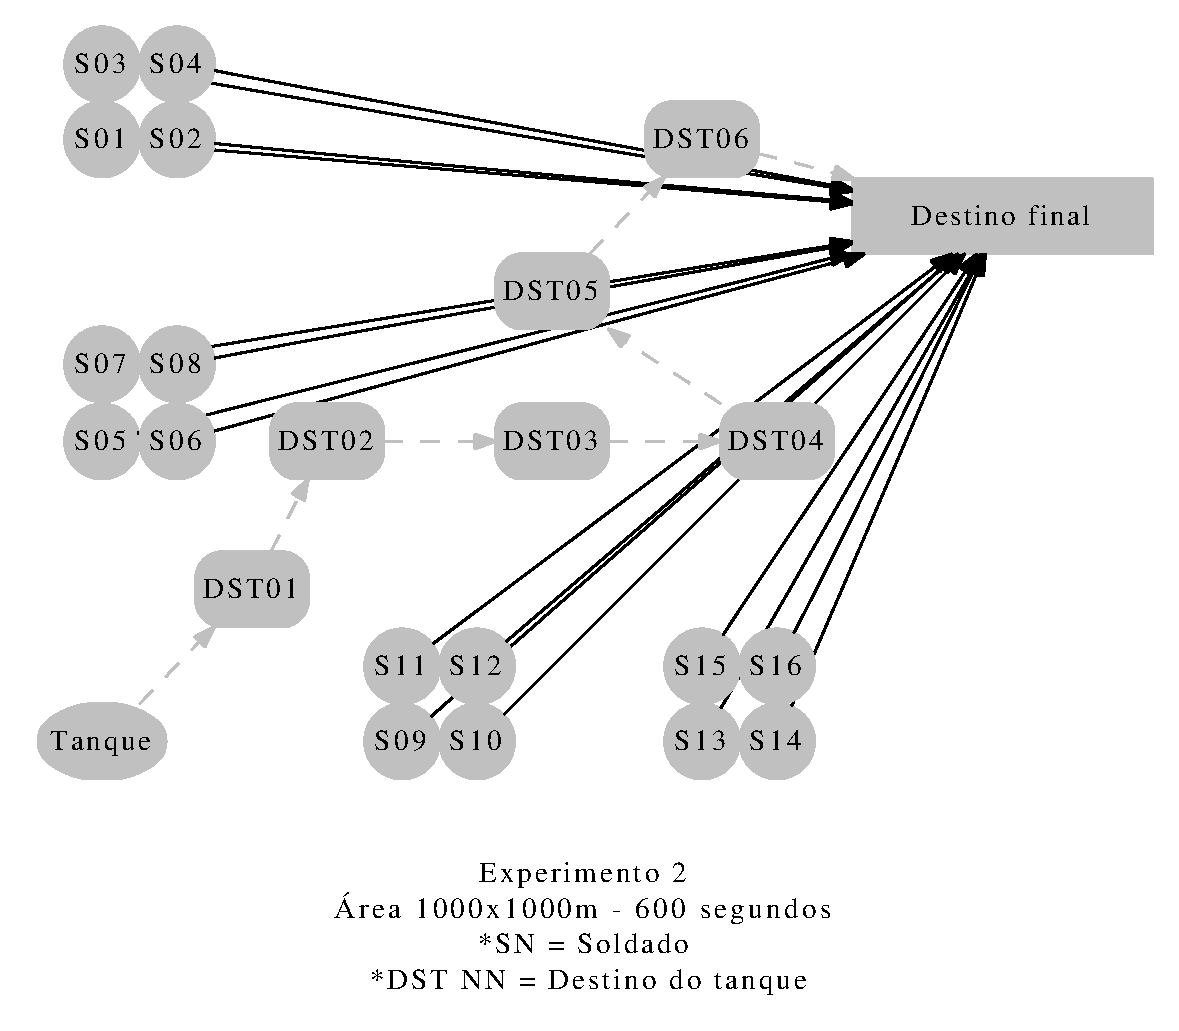
\includegraphics[scale=0.5]{experimento2.eps}
	\caption{Experimento 2}
	\label{figExp2}
\end{figure}

Todos os soldados de cada grupo dever\~ao avan\c{c}ar juntos durante o percurso do cen\'ario, n\~ao executando necessariamente um caminho em linha reta durante todo o trajeto.

A Tabela \ref{tabParamExp2} demonstra resumidamente os par\^ametros utilizados nesse experimento. 
Al\'em do tamanho, n\'umero de conex\~oes e n\'os diferentes do Experimento 1, podemos verificar que a velocidade dos n\'os possuem uma varia\c{c}\~ao.
Essa varia\c{c}\~ao ocorre pelo fato de que, os soldados recebem ordens de parada ou avan\c{c}o no percurso, sendo que em cada situa\c{c}\~ao \'e necess\'ario aumentar, diminuir ou at\'e mesmo parar o ritmo de avan\c{c}o no objetivo do cen\'ario.

\begin{table}[H]
	\centering
	\caption{Resumo dos par\^ametros usados no Experimento 2.}
	\begin{tabular}{ | l | l | }
		\hline
		N\'umero total de n\'os & 17 \\ \hline
		N\'umero de fontes de tr\'afego & 7 \\ \hline
		N\'umero de conex\~oes & 16 \\ \hline
		Tempo de simula\c{c}\~ao & 600 segundos \\ \hline
		\'Area total da simula\c{c}\~ao & 1000x1000 metros \\ \hline
		Tamanho dos pacotes & 512 \textit{bytes} \\ \hline
		Velocidade dos n\'os & 0 \`a 8 m/s constante \\ \hline
		Velocidade de banda & 11Mbps/s \\ \hline
	\end{tabular}
	\label{tabParamExp2}
\end{table}

\subsection{An\'alise comparativa dos resultados}

\subsubsection{Experimento 1}
Esta se\c{c}\~ao apresenta os resultados obtidos da simula\c{c}\~ao do Experimento 1.
Conforme os dados apresentados na Tabela \ref{tabExp1Result}, \'e poss\'ivel analisar que o protocolo AODV, o qual tem o modo de funcionamento reativo, possui uma taxa de entrega superior ao protocolo DSDV, que funciona em modo pr\'o-ativo, e ambos s\~ao baseados em Vetor de Dist\^ancias. 

A diferen\c{c}a na taxa de entrega ocorre pelo fato do AODV buscar uma rota para o destino no tempo em que \'e necess\'ario comunicar com esse mesmo destino, e o DSDV atualiza as rotas em intervalos distintos de tempo.
Quando a topologia muda no experimento, ou seja, a conex\~ao do Soldado 1 com o Soldado 3 altera o salto, pelo Soldado 2, para o Soldado 4, \'e necess\'ario que o protocolo altere a rota de comunica\c{c}\~ao dos Soldados.
Tal altera\c{c}\~ao vai depender como o protocolo funciona, e nesse caso, o modo reativo foi superior ao pr\'o-ativo com base em Vetor de Dist\^ancias.

Na execu\c{c}\~ao do experimento com o DSDV, considerando quando a comunica\c{c}\~ao ocorre pr\'oximo ao tempo de mudan\c{c}a da topologia da rede, o mesmo protocolo ainda n\~ao atualizou suas rotas, ent\~ao encaminha a comunica\c{c}\~ao por uma rota inv\'alida, e descarta os pacotes da comunica\c{c}\~ao. E o AODV, em tempo de execu\c{c}\~ao, consegue detectar a mudan\c{c}a da topologia.

\begin{table}[H]
	\centering
	\caption{Resultado das simula\c{c}\~oes do Experimento 1}
	\begin{tabular}{ | c | c | c | c | }
		\hline
		M\'ETRICAS AVALIADAS & DSDV & AODV & OLSR \\ \hline
		Taxa de entrega & 92.98\% & 99.83\% & 98.43\% \\ \hline
		Atraso m\'edio (ms) & 10.7575 & 11.4837 & 11.3047 \\ \hline
		N\'umero de pacotes & 543 & 588 & 565 \\ \hline
		N\'umero de \textit{bytes} & 288896 & 312816 & 300580 \\ \hline
	\end{tabular}
	\label{tabExp1Result}
\end{table}

Entretanto, quando um protocolo possui um funcionamento pr\'o-ativo, por\'em sendo baseado em Estado de Enlace, que \'e o caso do OLSR, percebe-se que a taxa de entrega aumenta em rela\c{c}\~ao ao DSVD, que \'e baseado em Vetor de Dist\^ancias.
Esse aumento ocorre porque, quando a topologia da rede do Experimento 1 \'e modificada, a base Estado de Enlace detecta a altera\c{c}\~ao de conex\~ao dos n\'os vizinhos, atualizando suas tabelas de rotas, o que altera o intervalo de atualiza\c{c}\~ao das rotas.

O objetivo inicial desse experimento era analisar o tempo de converg\^encia entre os protocolos, o qual n\~ao foi muito significativo.
Analisando os resultados de Atraso M\'edio de cada protocolo, percebe-se que as diferen\c{c}as foram menores de 1 ms entre os protocolos de roteamento, todos trabalhando pr\'oximos a 11 milissegundos.

Comparando as \'ultimas duas m\'etricas de desempenho, sendo elas, n\'umeros de pacotes e n\'umento de \textit{bytes}, pode-se analisar que o DSDV teve uma melhor efici\^encia quanto ao uso da rede. 
Esse resultado deve-se ao fato de que o AODV duplica os pacotes de roteamento, e \cite{ramachandran} comenta que o AODV n\~ao reutiliza informa\c{c}\~oes de roteamento, at\'e mesmo em casos comuns de comunica\c{c}\~ao.
J\'a o DSDV, mesmo atualizando as tabelas de roteamento a cada instante de tempo, pode reutilizar informa\c{c}\~oes, diminuindo o n\'umero de pacotes de roteamento. 

Os resultados do protocolo OLSR podem ser explicados pelo fato de que o mesmo atualiza suas rotas quando o Estado de Enlace muda. Assim, aumenta um pouco o n\'umero de pacotes em rela\c{c}\~ao ao DSDV, por\'em se demonstra eficiente com rela\c{c}\~ao ao AODV pela sua caracter\'istica pr\'o-ativa.

\subsubsection{Experimento 2}
Diferentemente do Experimento 1, o Experimento 2 possui caracter\'isticas espec\'ificas de mobilidade, em que cada soldado no cen\'ario n\~ao vai percorrer um caminho cont\'inuo, e tamb\'em, n\~ao vai ter uma velocidade constante de avan\c{c}o para o objetivo final do cen\'ario.
Foram gerados e executados 15 simula\c{c}\~oes de cen\'arios, e obtendo-se assim, um resultado de m\'edia somat\'oria entre os dados extra\'idos.
A Tabela \ref{tabExp2Result} demonstra a m\'edia destes resultados obtidos no Experimento 2.

Analisando a m\'etrica de Taxa de Entrega dos pacotes na simula\c{c}\~ao, pode-se observar que houve uma invers\~ao de desempenho entre o DSDV e o AODV, se comparado com o Experimento 1, pois o DSDV teve um resultado superior ao AODV.
Esse resultado pode ser explicado com base no tamanho total da rede, o qual teve um aumento significativo no n\'umero de n\'os que comp\~oem a simula\c{c}\~ao.
Como o modo de funcionamento do DSDV \'e pr\'o-ativo, ele mant\'em as tabelas de rotas para a comunica\c{c}\~ao. Em contrapartida, o AODV ter\'a que descobrir a rota antes de comunicar, por ser um protocolo reativo.
Como a rede desse experimento \'e maior, \'e poss\'ivel analisar que, dependendo do destino desejado, o AODV pode levar muito tempo para criar a comunica\c{c}\~ao, descartando os pacotes.

Essas mesmas caracter\'isticas, pr\'o-ativa e reativa, influenciam nos resultados da m\'etrica de desempenho de Atraso M\'edio, o qual o DSDV tem um resultado superior ao AODV, sendo mais r\'apido para entregar os pacotes.
A mesma caracter\'istica pr\'o-ativa pode explicar o resultado do protocolo OLSR tanto para as m\'etricas Taxa de Entrega como para o Atraso M\'edio.

\begin{table}[H]
	\centering
	\caption{Resultado das simula\c{c}\~oes do experimento 2}
	\begin{tabular}{ | c | c | c | c | }
		\hline
		M\'ETRICAS AVALIADAS & DSDV & AODV & OLSR \\ \hline
		Taxa de entrega & 96.88\% & 90.37\% & 95.29\%  \\ \hline
		Atraso m\'edio(ms) & 8.15969 & 16.3527 & 6.88545  \\ \hline
		N\'umero de pacotes & 7407 & 7696 & 7483  \\ \hline
		N\'umero de \textit{MegaBytes} & 3.76 & 3.90 & 3.80  \\ \hline
	\end{tabular}
	\label{tabExp2Result}
\end{table}

Analisando as m\'etricas N\'umero de Pacotes e N\'umero de \textit{MegaBytes}, percebe-se que o DSDV tamb\'em foi superior em rela\c{c}\~ao ao AODV na efici\^encia de roteamento.
Esse resultado foi favorecido pela caracter\'istica pr\'o-ativa em um experimento com um maior n\'umero de n\'os, logo que o DSDV n\~ao precisa buscar toda a topologia da rede toda a vez que necessita comunicar com o destino, que \'e o caso do AODV. 
O mesmo pode-se dizer do protocolo OLSR, por\'em, ele resultou em um n\'umero maior de pacotes que o DSDV por causa da sua base em Estado de Enlace, atualizando as tabelas de roteamento a cada mudan\c{c}a de conex\~ao dos n\'os vizinhos.


	%Experimentos e resultados
\section{Conclus\~ao e trabalhos futuros}\label{conclusao}

As simula\c{c}\~oes apresentadas neste trabalho confirmam o fato de que cada protocolo apresenta vantagens e desvantagens, dependendo dos condi\c{c}\~oes que lhe s\~ao impostas, como no caso, o n\'umero de n\'os na rede. 
Nos cen\'arios com prop\'ositos militares, que utilizam redes \textit{ad hoc}com configura\c{c}\~ao hier\'arquica, a entrega dos pacotes de forma eficiente e r\'apida \'e de extrema relev\^ancia. 
O protocolo "ideal" atenderia a todas as restri\c{c}\~oes impostas pelas necessidades de comunica\c{c}\~ao em cen\'arios tipicamente militares, mas o que se p\^ode concluir \'e a apartir dos resultados alcan\c{c}ados \'e que cada um dos protocolos avaliados mostrou sua diferen\c{c}a em determinada m\'etrica ou condi\c{c}\~ao.

Entre os protocolos analizados, podemos ver que o DSDV e o AODV tiveram comportamento opostos nos 2 diferentes experimentos realizados, e que o OLSR manteve uma boa estabilidade entre ambos os experimentos.

Para futuras pesquisas, \'e sugerido que seja combinado algumas caracter\'isticas de protocolos, prevalecendo das situa\c{c}\~oes onde em que eles apresentam maiores vantagens que se adaptem aos cen\'arios propostos. 

		%Conclusão

%Referencias bibliograficas sao editadas no arquivo referencias/bibliografias.bib
\section{Refer\^encias bibliogr\'aficas}
%\bibliographystyle{sbc}
\bibliographystyle{abnt-alf}
\def\bibindent{0.5cm}
\renewcommand{\emph}{\textbf}
\bibliography{referencias}

\end{document}
